\documentclass[a4paper,11pt]{article}
\usepackage[utf8]{inputenc}
\usepackage[T1]{fontenc}
\usepackage[slovene]{babel}
\usepackage{amssymb}

\usepackage{a4wide}
\usepackage{fullpage}

\usepackage[toc,page]{appendix}
\usepackage[pdftex]{graphicx} % for figures
\graphicspath{ {../slike/} }
\usepackage[space]{grffile}
\usepackage{setspace}
\usepackage{color}
\definecolor{light-gray}{gray}{0.95}
\usepackage{hyperref}

\renewcommand{\baselinestretch}{1.2}



\usepackage{minted}
\usemintedstyle{pastie}
\fvset{tabsize=3,samepage=true,baselinestretch=1.22}
\setminted{linenos=true,numbersep=6pt,fontsize=\small}

\title{Izdelava modela letala pri predmetu Računalniško podprto geometrijsko oblikovanje}
\author{Rok Kralj (27142126)}
\date{\today}

\begin{document}
	\maketitle
	
	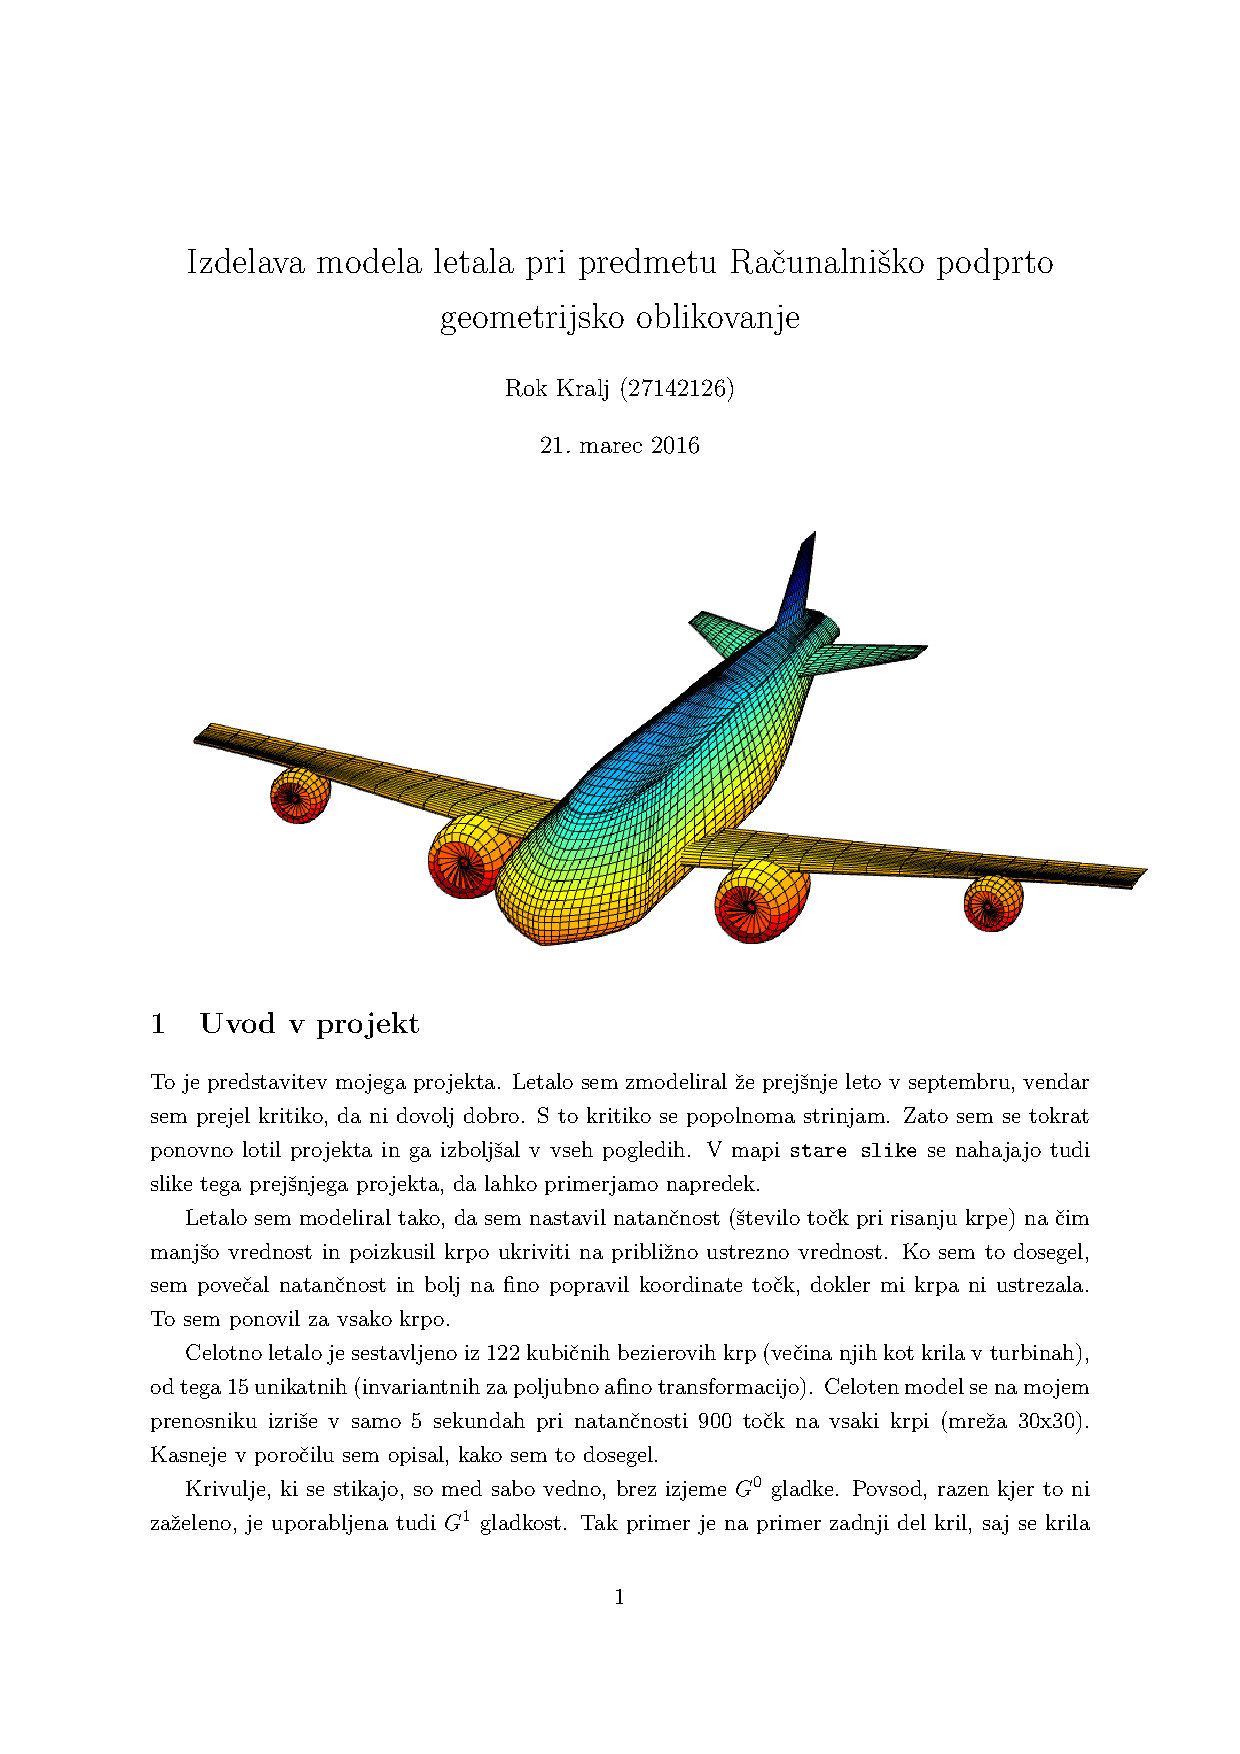
\includegraphics[scale=0.55]{letalo}
	
	\section{Uvod v projekt}
	
	To je predstavitev mojega projekta. Letalo sem zmodeliral že prejšnje leto v septembru, vendar sem prejel kritiko, da ni dovolj dobro. S to kritiko se popolnoma strinjam. Zato sem se tokrat ponovno lotil projekta in ga izboljšal v vseh pogledih. V mapi \texttt{stare slike} se nahajajo tudi slike tega prejšnjega projekta, da lahko primerjamo napredek.
	
	Letalo sem modeliral tako, da sem nastavil natančnost (število točk pri risanju krpe) na čim manjšo vrednost in poizkusil krpo ukriviti na približno ustrezno vrednost. Ko sem to dosegel, sem povečal natančnost in bolj na fino popravil koordinate točk, dokler mi krpa ni ustrezala. To sem ponovil za vsako krpo.
	
	Celotno letalo je sestavljeno iz 122 kubičnih bezierovih krp (večina njih kot krila v turbinah), od tega 15 unikatnih (invariantnih za poljubno afino transformacijo). Celoten model se na mojem prenosniku izriše v samo 5 sekundah pri natančnosti 900 točk na vsaki krpi (mreža 30x30). Kasneje v poročilu sem opisal, kako sem to dosegel.
	
	Krivulje, ki se stikajo, so med sabo vedno, brez izjeme $G^0$ gladke. Povsod, razen kjer to ni zaželeno, je uporabljena tudi $G^1$ gladkost. Tak primer je na primer zadnji del kril, saj se krila v prerezu zožajo proti koncu.
	
	Posebno pozornost sem posvetil izdelavi turbin, saj sem moral aproksimirati krog z Bezierovo krivuljo, prav tako pa sem izdelal krila v turbinah. Potrudil sem se, da si nisem podvojeval dela, zato sem krpe zrcalil, premikal in obračal.
	
	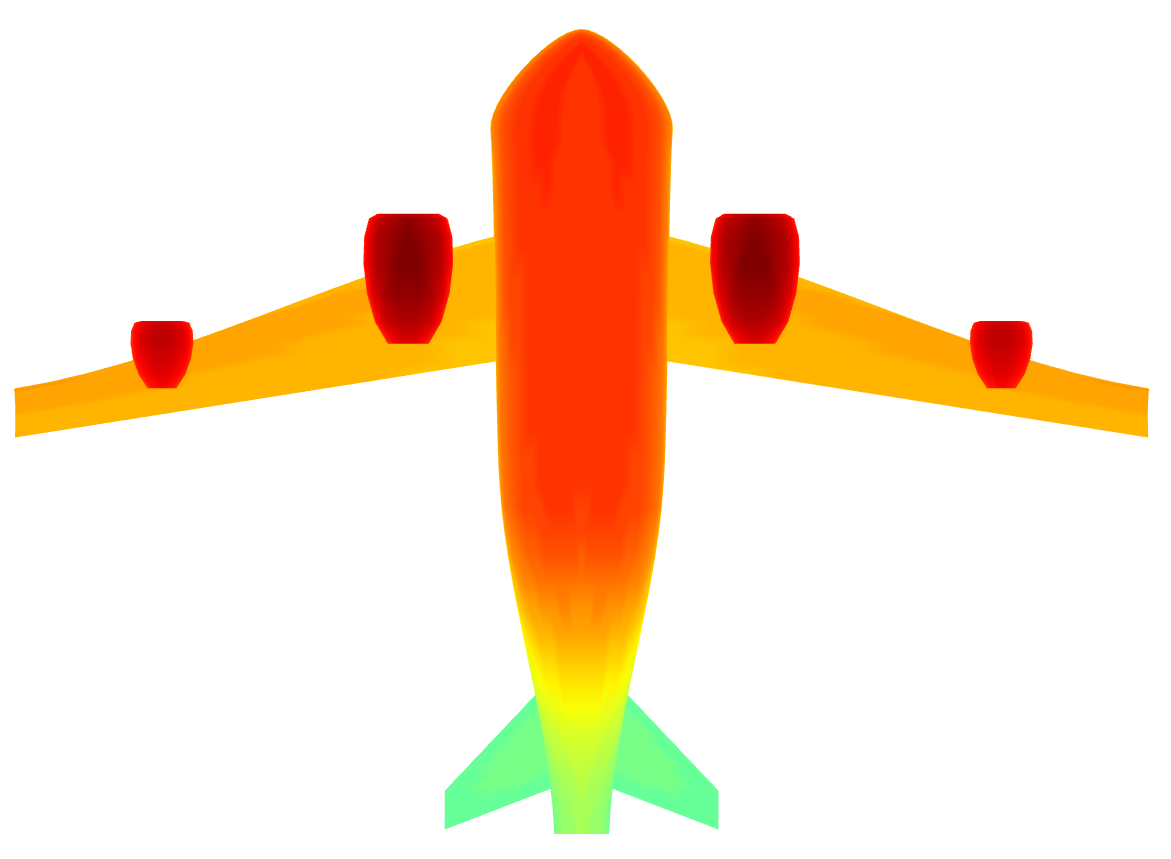
\includegraphics[scale=0.35]{spodaj}
		
	\subsection{Poganjanje projekta in tehnične stvari}
	
	Za ogled objekta moramo pognati \texttt{projekt.m}. V tej datoteki lahko tudi nastavimo natančnosti risanja, ki pa je že nastavljena na smiselno vrednost. Tudi kot kamere je nastavljen na ustrezno vrednost.
		
	Projekt je bil napisan v Octave verzije 4.0.0, zato je mogoče, da v okolju MATLAB ne bo deloval, saj se dva občasno malo razlikujeta. Prav mogoče je tudi, da je program hitrejši, če ga poženemo v MATLABU namesto v Octave-u.
	
	\section{Organizacija programske kode in krp}
	
	\subsection{Vrste krp}
	
	Končni model letala vsebuje kubične Bezirerove krpe dveh vrst.
	
	Prva vrsta krp je vsebovana v datotekah, ki se začnejo s podčrtajem in se končajo s končnico \texttt{.krpa}. Te datoteke se da odpreti in pregledovati v vsakem urejevalniku besedila. Vsaka taka datoteka vsebuje tri 4x4 matrike ena pod drugo, ločene s prazno vrstico (vsaka matrika predstavlja eno izmed dimenzij). Te datoteke sem urejal na roke, tudi zveznosti sem računal na roko. Napisal sem tudi funkcijo \texttt{nalozi()}, ki tako datoteko naloži v pomnilnik.
	
	Druga vrsta krp pa je generirana, to so torej MATLAB funkcije, ki sprejmejo neke parametre in vrnejo polje treh matrik. Na primer pri aproksimaciji kroga je bolje, da so točke predstavljene s čim bolj natančnim zapisom v plavajoči piki, kar pa bi težko dosegel na prvi način.
	
	Obe predstavitvi Bezierovih krp program obravnava enako ko sta enkrat naloženi v pomnilnik.
	
	\subsection{Združevanje krp v končni objekt}
	
	V glavnem imeniku se nahaja datoteka \texttt{projekt.m}, ki vsebuje funkcijo, ki s pomočjo nalaganja prej omenjenih krp sestavi končni objekt. Pri tem si pomaga z afinimi transformacijami. Ta datoteka je precej obsežna, okoli 200 vrstic, saj združi vse elemente skupaj.
	
	V tej datoteki lahko nastavimo tudi natančnost, torej gosto mreže v vsaki dimenziji. 
	
	\subsection{Računanje Bezierovih ploskev}
	
	Kasneje v poročilu sem opisal, kako se mi je uspelo izogniti uporabi trikotnih bezierovih krp. Torej je celoten model sestavljen iz kubičnih bezierovih krp, zato se lahko omejimo na učinkovito risanje teh.
	
	Ko sem začel s projektom, sem najprej napisal De Casteljauov algoritem. Ker sem potreboval čim hitrejše risanje ploskev zaradi v uvodu opisanega postopka dela (torej popravi, nariši, ponovi), sem implementiral bolj učinkovit algoritem prek matrične oblike Bezierove krivulje. Kasneje sem ga izboljšal še tako, da določen del račuanja predpomnim izven zank in ne ponavljam v vsaki iteraciji.
	
	Hitrejše izvajanje algoritma se mi zdi da odpade na to, da lahko računalnik uporabi učinkovite BLAS metode pri množenju matrik, česar pa ne more pri \texttt{for} zankah in računanju po stoplcih. Vektorizacija se skoraj vedno izplača. Kasneje sem še ročno prevedel Octave s knjižnico OpenBLAS, vendar se mi zdi, da to ni preveč pomagalo.
	
	Funkcijo, ki deluje za poljubno dimenzionalne prostore (ne samo 3, kot v našem primeru) zaradi svoje elegantnosti prilagam kar v poročilo.

\begin{minted}{octave}
function Q = krpa(P, natancnost)
	if nargin < 2
		natancnost = 20;
	end
	
	% funkcija deluje za poljubno dimenzionalne prostore
	dimenzij = size(P, 3);

	% popraviti, če žeimo kakšno neenakomerno mrežo
	u = v = linspace(0, 1, natancnost);

	% zapis v matrični obliki
	M = [
		1   0   0   0;
	   -3   3   0   0;
		3  -6   3   0;
	   -1   3  -3   1
	];
	
	% predpomnimo matriko za vsako izmed dimenzij
	% da ne množimo v vsaki iteraciji
	for k = 1:dimenzij
		A{k} = M * P(:,:,k) * M';
	end

	potence = @(v) [1, v, v*v, v*v*v];

	% izračunamo vse točke mreže
	for i = 1:natancnost
		U = potence(u(i));
		for k = 1:dimenzij
			x = U * A{k};
			for j = 1:natancnost
				V = potence(v(j));
				Q(i,j,k) = x * V';
			end
		end
	end
\end{minted}

Mogoče ste opazili pametno postavitev \texttt{for} zank v zadnjih nekaj vrsticah, zanki za spremenljivki $k$ in $j$ sta namreč zamenjani. To nam omogoči, da vmesni rezultat shranimo v spremenljivko $x$ in tako naredimo reda \texttt{natancnost} manj matrično-vektorskih množenj, kar se zelo pozna. Za vsako točko imamo torej amortizirano samo en skalarni produkt magnitude 3 (v našem primeru), kar je res hitro.

Za še večjo učinkovitost bi se dalo še predpomniti rezultate klica funkcije \texttt{potence()} v najbolj notranji zanki.
	
	\subsection{Afine transformacije}
	
	Napisal sem kar nekaj funkcij, ki delajo afine preslikave. Vse te funkcije sprejmejo eno krpo (torej tri matrike). V tej predstavitvi je potrebno nekaj razmišljanja, kako pripraviti, da vse skupaj pravilno deluje. Primer rotacije vzdolž X osi prilagam spodaj:
	
	\begin{minted}{matlab}
function K = rotacijaXplane(Q, kot)
	K(:, :, 1) = cos(kot)*Q(:, :, 1) + sin(kot)*Q(:, :, 3);
	K(:, :, 3) = -sin(kot)*Q(:, :, 1) + cos(kot)*Q(:, :, 3);
	K(:, :, 2) = Q(:, :, 2);
	\end{minted}
	
	Primeri ostalih afinih transformacij, ki sem jih napisal so zrcaljenje, skrčitev, rotacija okrog različnih osi in traslacija za nek vektor. Ostalih nisem potreboval oziroma so tako ali tako kompozicija naštetih operacij (razen striga, seveda).
	
	
	\section{Zanimiv del projekta: Ustvarjanje turbine}
	
	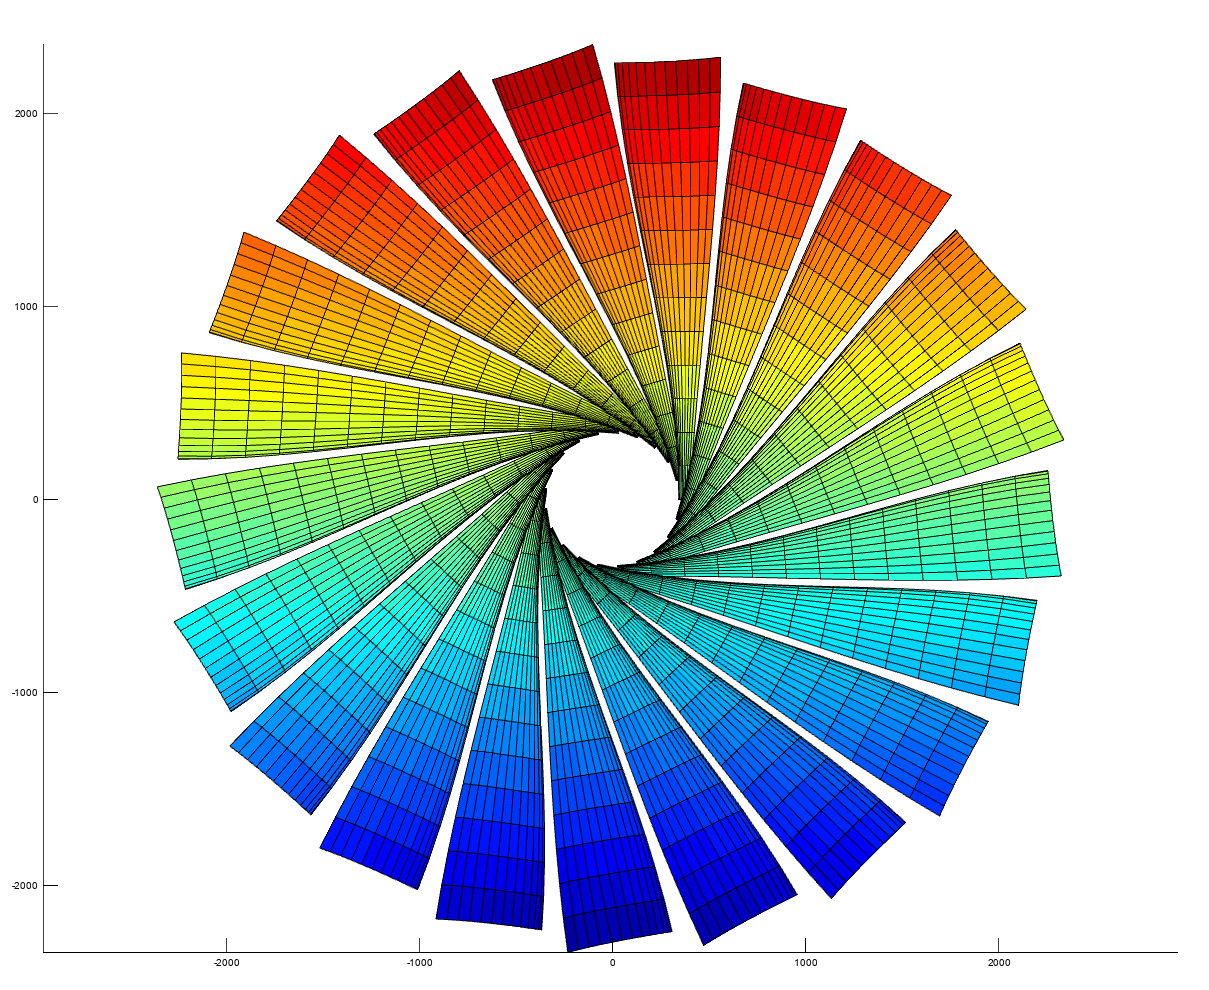
\includegraphics[scale=0.35]{krilca v turbini}
	
	Pri izdelavi turbine je bila prva stvar, ki sem se je lotil, izdelava krilc, ki poskrbijo za pretok zraka. Zaradi tega morajo imeti specifično obliko, saj morajo zrak zajemati in ga odrivati nazaj. To je še bolje vidno iz stranske perspektive:
	
	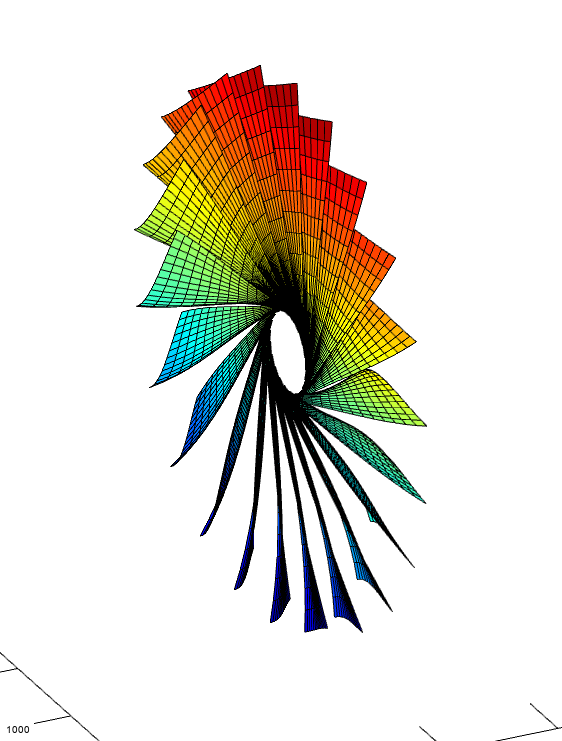
\includegraphics[scale=0.45]{krilca v turbini 2}
	
	Seveda sem tudi tukaj naredil samo eno izmed krilc, ostale pa sem v kodi še devetnajskrat obrnil za sorazmeren kot, pri tem pa pustil še nekaj prostora v sredini.

	
	\subsection{Aproksimacija kroga z Bezierovimi konstrukti}
	
	Sedaj pa je bil na vrsti težji del, in sicer aproksimacija krožnice z Bezierovo krivuljo. Znano je, da je z Bezierovimi krivuljami nemogoče doseči popolno prileganje krožnici (pod pogojem, da uporabimo končno število njih). Racionalizacijo za to nam lahko da De Casteljauov postopek, saj nam kot točke na krivulji vedno vrača samo racionalna števila, vemo pa, da je to res samo za nekatere točke na krožnici. Nemogoče je to torej, da bi Bezierova krivulja pravilno določila vse točke krožnice.
	
	Ker bi dobili zelo slabo aproksimacijo, če bi se odločili, da celoten obseg aproksimiramo samo z eno kubično krivuljo, običajno postopamo tako, da krožnico razdelimo na $K \geq 4$ enakih lokov, zmodeliramo enega izmed njih, ostale pa dodamo z rotacijo.
	
	Celoten algoritem je mogoče videti v datoteki \texttt{aproksimacijaKroga.m}, ki nam vrne kontrolne točke kubične bezierove krivulje za eno četrtino krožnice. Te točke lahko kasneje uporabimo pri generaciji kubičnih bezierovih ploskev. Tukaj prilagam še kratko izpeljavo formule in mere za napako.
	
	Pri kubični bezierovi krivulji imamo na voljo 4 točke, recimo jim $A, B, C, D \in \mathbb{R}^2$. Dve porabimo za to, da dosežemo $C^0$ zveznost, se pravi da se loki držijo skupaj. Točki $A, D$ torej eksaktno interpolirata krožnico na enakomernem kotu.
	
	Naprej želimo na stikih $C^1$ zveznost, to poemeni, da se smer in dolžina tangent ujemata, to pa je mogoče samo takrat, ko sta obe tangenti pravokotni na radij. Ko vse to premislimo, uvidimo, da imamo na voljo samo eno prostorsko stopnjo $d$, torej $d = ||A - B||_2 = ||C - D||_2$. Sedaj pa si poglejmo, kako določimo optimalen $d$ za dano mero napake. Za lažjo izpeljavo, si izberimo kokreten primer, ko število lokov $K = 4$, saj so v tem primeru tangente vzporedne s koordinatnimi osmi. Kontrolne točke so torej sledeče:
	$$
		A = (0, 1),
		B = (d, 1),
		C = (1, d),
		D = (1, 0).
	$$
	
	Kar privede do naslednje parametrične enačbe za lok:
	
	$$
		f_x(t) = 3t(1-t)^2d + 3t^2(1-t)+t^3
	$$
	$$
		f_y(t) = (1-t)^3 + 3t(1-t)^2 + 3t^2(1-t)d
	$$
	
	Za mero za napako si bomo izbrali kar $L_1$ napako, torej $e(t) = \sqrt{f^2_x(t) + f^2_y(t)} - 1$. Na tej točki sem hotel napako minimizirati enakomerno, torej izračunati določeni integral mere za napako kvadrirane za $0 \leq t \leq 1$, vendar se to ni obneslo. Zato bomo poračunali maksimume in minimume funkcije napake ter tako minimizirali absolutno vrednost.
	
	Izkaže se, da je minimum funkcije, ne glede na $d$, vedno pri $t = \frac{1}{2}$, njegova vrednost pa je
	$$
		e_{min} = e\left(\frac{1}{2}\right) = \sqrt{\frac{9 d^2+24 d+16}{32}} - 1.
	$$.
	
	Maksimum pa je dosežen v dveh točkah, ampak ima obakrat isto vrednost:
	$$
		e_{max} = e\left(\frac{1}{2} \pm \frac{12-20d-3d^2}{4-6d}\right) = \frac{3d-1}{(3 d-2)^2}\sqrt{8 - 24 d + 12 d^2 + 8 d^3 + 3 d^4}-1.
	$$
	
	Vemo, da bomo najbolje optimizirali napako, ko bosta maksimum in minumum funkcije napake ravno nasprotna, torej mora veljati
	$$
		e_{min} = -e_{max},
	$$
	kar pa nima algebraično izražljive rešitve (je ena izmed ničel polinoma stopnje 12) in je blizu $d \approx 0.55191502449351057074$, kar je tudi konstanta, vprogramirana v moj program, saj sem jo naračunal na toliko decimalk, da zadosti IEE v dvojni natančnosti. Sedaj, ko imamo konstanto končno izračunano tako, da krivulja kar se da malo odstopa od krožnice, lahko turbino še narišemo:
	
	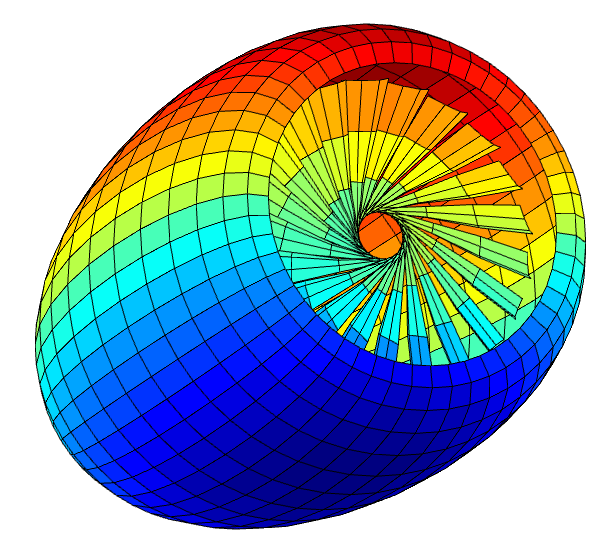
\includegraphics[scale=0.55]{turbina}
	
	\section{Kaj bi se dalo še narediti?}
	
	Zaenkrat je letalo glede na višino pobarvano z barvami mavrice. Moj prvotni namen je bil tudi, da bi poskusil površine teksturizirati, torej v nekem grafičnem programu ustvari primerne teksture z elementi, ki jih običajno vidimo na zunanjosti letala, kot na primer lučke, okna, logotipe letalskih družb. Kasneje sem spoznal, da je to težje in bolj zamudno kot sem misli, poleg vsega pa Octave tega zaenkrat še ne omogoča.
	
\end{document}
